\chapter{Variational Lenses}\label{sec:configlenses}
In this section we present a new lens definition building on the formalisations 
of the \emph{put} and \emph{get} operators we have created in the previous
section. We will expand on the lenses we have introduced in Section~\ref{sec:background:lenses}.

\noindent\emph{Configuration.}
If we want to constrain our \emph{get} and \emph{put} operators from
Sections \ref{sec:vp:getoperator} and \ref{sec:vp:putoperator} into a lens, we
need to create a new kind of lens. The reason is that the typing of the
standard lenses constrict us too much to be able to fit our
operators.

To allow for this new lens to be applicable beyond the scope of the Virtual
Platform, we extract more general types from our formalisations of the
operators:
\[
  \begin{array}{lll}
    \textit{get} & : & \binaryFunc{C}{E}{A} \\
    \textit{put} & : & \ternaryFunc{D(A)}{C}{E \times E}{C} \\
    \textit{create} & : & \binaryFunc{A}{E}{C}
  \end{array}
\]
The \emph{get} function now takes two arguments, first we see the concrete
structure as we have seen it before, but now it comes with an \(E\): this part
carries the configuration information (in our case, the expression or choice.)
The result of the \emph{get} function still is the abstract structure as before. Note
that we \emph{will} show the definitions of the \emph{create} functions here, 
but we will not go into the implementations of this function. This implementation
would involve the creation of a new system in the Virtual Platform starting from an
existing codebase.

The \emph{put} function changes similarly, we still see the concrete
argument, and we have again added configuration arguments. We both have the 
configuration argument that was applied to the \emph{get} operator (the
\emph{choice}) and the configuration used in the \emph{put} operator, which for
us is the \emph{ambition}. The most important change here is that the abstract
argument has changed into \(D(A)\). This \(D\) stands for \emph{diff}, as we
need the abstract argument combined with some sort of diffing structure. This
can be seen as a list of changes made to the view. What
is important is that we need to have a function
\(\textit{empty} : \unaryFunc{A}{D(A)}\) that can transform an abstract
structure into a diffing structure. This function should, as the name suggests,
deliver an empty diff structure. We will use this function in new lens laws.

Finally, we have the \emph{create} function, this function has changed from the
original in the same way the \emph{get} function changed, we have only added a
configuration argument \(E\) to it.

Since we have changed the signature of the lens functions, we also have to
adapt the lens laws accordingly:
\[
  \begin{array}{ll}
    \mathit{put}\left(\mathit{empty}\left(\textit{get}~c~e\right)\right)~c~e~e = c & \getput \\
    \mathit{get}\left(\mathit{put}(d(a)~c~e_g~e)\right)~\left(e\otimes e_g\right) = a & \putget \\
    \mathit{get}\left(\mathit{create}~a~e\right)~e = a & \createget
  \end{array}
\]
Here, we have that \(e_g\) is the configuration used to get to the view, which
is put back using the \emph{put} function. How the first two laws interact with
the system as a whole can also be seen in Figure \ref{fig:operator:overview}.

\begin{figure}
  \centering
  \resizebox{0.5\textwidth}{!}{%
  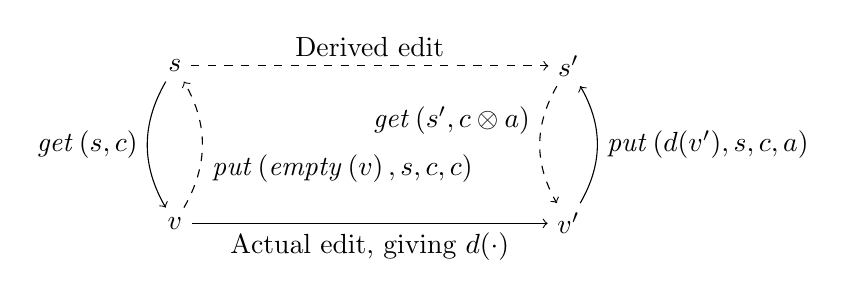
\begin{tikzpicture}
    \node[] (OS) at (0, 2) {$s$};
    \node[] (OV) at (0, 0) {$v$};
    \node[] (ES) at (5, 2) {$s'$};
    \node[] (EV) at (5, 0) {$v'$};
    
    \draw[dashed,->] (OS) -- (ES) node [midway, above] {Derived edit};
    \draw[->] (OV) -- (EV) node [midway, below] {Actual edit, giving $d(\cdot)$};
    \path[->] (OS) edge[bend left=-30] node[left] {$\mathit{get}\left(s, c\right)$} (OV);
    \path[dashed,->] (ES) edge[bend left=-30] node[left, yshift=3mm] {$\mathit{get}\left(s', c \otimes a\right)$} (EV);
    \path[dashed,->] (OV) edge[bend right=30] node[right, yshift=-3mm] {$\mathit{put}\left(\mathit{empty}\left(v\right), s, c, c\right)$} (OS);
    \path[->] (EV) edge[bend right=30] node[right] {$\mathit{put}\left(d(v'), s, c, a\right)$} (ES); 
  \end{tikzpicture}
  }%
  \caption{Overview of operator relationships.}
  \label{fig:operator:overview}
\end{figure}

\subsection*{Virtual Platform}\label{sec:configlenses:vp}
We want to work towards proving the defined lens laws for our instance of the
lens. Before we start working on that, let us first look at how we
should fill in the abstract types in order to fit our \emph{get} and \emph{put}
functions:
\[
  \begin{array}{l}
    C = \allassets \\
    E = \expressions{\features} \\
    A = \optional{\allassets} \\
    D(A) = \optional{\allassets} \times \powerset{\allidentities}
  \end{array}
\]
Indeed, if we fill in these types for the different functions we get:
\[
  \begin{array}{lll}
    \textit{get} & : & \binaryFunc{\allassets}{\expressions{\features}}{\optional{\allassets}} \\
    \textit{put} & : & \ternaryFunc{\optional{\allassets} \times \powerset{\allidentities}}{\allassets}{\expressions{\features} \times \expressions{\features}}{\allassets} \\
    \textit{create} & : & \binaryFunc{\optional{\allassets}}{\expressions{\features}}{\allassets}
  \end{array}
\]

We want to minimise the restrictions put on the ambition in the \emph{put}
operator. But if we want to stay true to the lens laws defined just above, we
need at least some limitation, to illustrate the issue, see Figure
\ref{fig:operator:vp:example}. This example is structured much like in Figure
\ref{fig:operator:overview}, where we start in the top-left corner and work our
way to the top-right corner. We start with an asset tree with three
children, with $A$, $\neg B$ and $\neg A$ as presence conditions respectively.
To get our view, we take the entire tree and \emph{get} it using $A$ as our
choice expression. This leads to the removal of the third child as 
$\neg A \land A \not\in \sat$. Next, we edit our view such that $a_1$ is
changed and $a_4$ is added. Finally, we want to \emph{put} our new asset tree
back into the original asset tree. To do this, we choose as ambition expression
just $B$. Note that the changed asset set contains $a_1$ and $a_4$, for now, we
assume that the identities of the assets $a_1$ and $a_4$ have the same name.
The result of our operation is as expected, we now have two versions of $a_1$,
one is the original ($a_1$) and the new one is the edited version ($a'_1$). We
also see that $a_4$ now has $B$ as its presence condition and that it is placed
after the previously hidden $a_3$. Now, we run into the following problem: the
\putget~ law says that we need to have some expression $e$ such that
\(\textit{get}\left(r_3, e\right) = r'_2\). Currently, this is not possible, as
we want both $a'_1$, $a_2$ and $a_4$ in our result. In other words, we do not
want $a_1$ and $a_3$. The way to do this is to choose $e = A \land B$. This
does not work for us though, as it would lead to $r'_2$ without $a_2$, as 
$\neg B$ would not hold anymore.

The example shows that we need some limitation in terms of what expression you
can choose for the ambition. To satisfy the lens laws we restrict the ambition
in the \emph{put} operator in the following way: for every asset $a$ in $\newassets$, with
\emph{am} being the ambition and \emph{ch} being the choice expression:
\[
  \mathit{ch} \land \mathit{am} \land \presenceconditionfunc(a) \in \sat
\]
This says that the choice expression, together with the ambition and any asset
presence condition must be satisfiable. We will now show that this limitation
indeed makes our definition of \emph{put} adhere to the lens laws.

\begin{figure}
  \centering
  \resizebox{0.6\textwidth}{!}{%
  \begin{tikzpicture}
    \node[] (T1R) at (0, 2) {$r_1$};
    \node[] (T1A1) at (-1,1) {$a_1$};
    \node[] (T1A2) at (0,1) {$a_2$};
    \node[] (T1A3) at (1,1) {$a_3$};
    \draw[] (T1R) -- (T1A1.north) node [midway, left, yshift=1mm] {$A$};
    \draw[] (T1R) -- (T1A2.north) node [midway, right, xshift=-1mm] {$\neg B$};
    \draw[] (T1R) -- (T1A3.north) node [midway, right, yshift=1mm] {$\neg A$};

    \node[] (T2R) at (0, -1) {$r_2$};
    \node[] (T2A1) at (-.5,-2) {$a_1$};
    \node[] (T2A2) at (.5,-2) {$a_2$};
    \draw[] (T2R) -- (T2A1.north) node [midway, left, yshift=1mm] {$A$};
    \draw[] (T2R) -- (T2A2.north) node [midway, right, yshift=1mm, xshift=-1mm] (T2ANCH) {$\neg B$};

    \node[] (T3R) at (6,-1) {$r'_2$};
    \node[] (T3A1) at (5,-2) {$a_1$};
    \node[] (T3A2) at (6,-2) {$a_2$};
    \node[] (T3A4) at (7,-2) {$a_4$};
    \draw[] (T3R) -- (T3A1.north) node [midway, left, yshift=1mm] (T3ANCH) {$A$};
    \draw[] (T3R) -- (T3A2.north) node [midway, right, xshift=-1mm] {$\neg B$};
    \draw[] (T3R) -- (T3A4.north) node [midway, right, yshift=1mm, xshift=-1mm] {};

    \node[] (T4R) at (6,2) {$r_3$};
    \node[] (T4A1) at (4,1) {$a_1$};
    \node[] (T4A1E) at (5,1) {$a'_1$};
    \node[] (T4A2) at (6,1) {$a_2$};
    \node[] (T4A3) at (7,1) {$a_3$};
    \node[] (T4A4) at (8,1) {$a_4$};
    \draw[] (T4R) -- (T4A1.north) node [midway, left, yshift=1mm] {${\scriptstyle A \land \neg B}$};
    \draw[] (T4R) -- (T4A1E.north) node [midway, right, xshift=-2mm, yshift=-1mm] {${\scriptstyle A \land B}$};
    \draw[] (T4R) -- (T4A2.north) node [midway, right, xshift=-1mm] {${\scriptstyle \neg B}$};
    \draw[] (T4R) -- (T4A3.north) node [midway, right, xshift=1mm, yshift=-1mm] {${\scriptstyle \neg A}$};
    \draw[] (T4R) -- (T4A4.north) node [midway, right, yshift=1mm] {${\scriptstyle B}$};

    \draw[double,-Stealth] (T1A2) -- (T2R) node [midway, left] {$\textit{get}\left(r_1, A\right)$};
    \draw[double,-Stealth] (T2ANCH) -- (T3ANCH) node [midway, below] {Edit $a_1$, add $a_4$};
    \path[] (T3R) edge[double,-Stealth,bend right=30] node[right] {$\textit{put}\left(r'_2, \left\{ a_1, a_4 \right\}, r_1, A, B\right)$} (T4A2); 
    \path[] (T4A2) edge[dashed,double,-Stealth,bend left=-30] node[left] {$\textit{get}\left(r_3, ?\right)$} (T3R); 
  \end{tikzpicture}
  }%
  \caption{Example of relationships between lens operators on the Virtual Platform showing why we need a restriction on the ambition expresion.}
  \label{fig:operator:vp:example}
\end{figure}

\subsection*{Proving the lens laws}
We want to show that the proposed lens laws hold for the formalisation of the
operators created for the virtual platform. We will start with the \getput~ law
and then prove the \putget~ law.

\begin{theorem}
  The formalisations of \emph{get} and \emph{put} in Sections~\ref{sec:vp:getoperator}
  and \ref{sec:vp:putoperator} adhere to the \getput~ law.
\end{theorem}

\begin{proof}
  As we know, the \getput~ law says that when we use the \emph{put} operator
  directly after the \emph{get} operator, we should result in the same asset
  tree. Our law uses an empty function that needs to be defined on the $D(A)$
  type. So in our case we need a function
  \(\textit{empty} : \unaryFunc{\optional{\allassets}}{\optional{\allassets} \times \powerset{\allidentities}}\).
  This is a simple function that takes an optional asset and returns that asset
  in combination with an empty set. So \(\textit{empty}~x = x, \emptyset\).
  By definition, the \emph{put} operator only makes changes to assets in the
  set of changed assets. Our \emph{empty} function always creates an empty set of
  changes and thus no changes will be applied. This ultimately means that the
  result of the \emph{put} operator, when applied with an empty change set, will
  always be the concrete argument given to it. This is even stronger than the
  lens law we need to prove: in our method, the ``ambition'' argument to the function
  may even differ from the ``choice'' argument:
  \[
    \mathit{put}\left(\mathit{get}~c~e_1\right)~\emptyset~c~e_1~e_2 = c
  \]
  This proves that the \getput~ law is always satisfied.
\end{proof}

\begin{theorem}
  The formalisations of \emph{get} and \emph{put} in Sections~\ref{sec:vp:getoperator}
  and \ref{sec:vp:putoperator} adhere to the \putget~ law.
\end{theorem}

\begin{proof}
  The \putget~ law states that we should be able to get back to a possibly edited
  view from the result of the \emph{put} operator applied on that edited view. We
  of course know the typing of the operators on the Virtual Platform and thus can
  fill in our definitions of $d(a)$ and $\otimes$. The $d(a)$ we can replace with
  two arguments, one for the asset ($a$) and one for the set of changed assets
  ($\powerset{\allidentities}$). The binary operator combining the configurations
  is replaced with the conjunction operator ($\land$):
  \[
    \mathit{get}\left(\mathit{put}(a~i~c~e_g~e)\right)~\left(e\land e_g\right) = a
  \]
  We start off by stating that all assets $a'$ in the tree of $a$ have a presence 
  condition such that:
  \begin{equation}\label{eq:vp:get:pclimitation}
    e_g \land \presenceconditionfunc(a') \in \sat
  \end{equation}
  We know this since that is what the \emph{get} operator used to retrieve the
  assets. 
  And by the restriction we introduced earlier, we also know that all assets $a'$
  in the tree of $a$ have that just \emph{before} applying the \emph{put}
  operator:
  \begin{equation}\label{eq:vp:put:ambitionrestriction}
    e_g \land e \land \presenceconditionfunc(a') \in \sat
  \end{equation}
  If this does not hold for any of the assets in the tree, we cannot apply the
  operator. Note that this second equation is a stronger version of the first
  one. Also note that this second equation contains $e_g \land e$, which is
  exactly what the \emph{get} operator in the law uses to obtain the result. This
  means that all the assets that are visible in $a$ will also be obtained after
  applying the \emph{get} operator. But since the \emph{put} operator can change
  the presence conditions of the assets, we have to look at the possible changes
  it can make before we can conclude that the law holds.
  \begin{enumerate}
    \item If an asset was edited, we want that after the \emph{get} operator, the
          edited version is visible, not the original version of that asset. We
          are sure that this will happen since:
          \begin{itemize}
            \item The ``old'' asset used to satisfy (\ref{eq:vp:get:pclimitation}),
                  but will be changed such that the presence condition of it is
                  combined with the negation of the ambition ($\neg e$), that
                  means that the new presence condition can never satisfy the
                  \emph{choice} expression of the final \emph{get} operator.
            \item The ``new'' asset already satisfied (\ref{eq:vp:put:ambitionrestriction})
                  before applying the \emph{put} operator, and it will only be
                  changed such that the ambition is combined with the ambition
                  ($e$), this means that (\ref{eq:vp:put:ambitionrestriction}) will
                  keep holding.
          \end{itemize}
    \item If an asset was added, it satisfied (\ref{eq:vp:put:ambitionrestriction})
          before the \emph{put} operator, and it will only get the ambition ($e$)
          added to its presence condition, so similar to what we have seen
          before, (\ref{eq:vp:put:ambitionrestriction}) will keep holding. This
          means that the added asset will indeed be in the result of the
          \emph{get} operator.
    \item If an asset was deleted, the ``old'' asset used to satisfy (\ref{eq:vp:get:pclimitation}),
          but similarly to what we have seen before, this asset cannot be in the
          result of the \emph{get} operator, since it gets the negation of the
          ambition ($\neg e$) appended to its presence condition.
  \end{enumerate}
  This means that any changes in the asset tree cannot lead to the assets not
  being in the result of the \emph{get} operator. We now still have to show that
  any assets that did not show up after the initial \emph{get} operator, will also
  not be in the result of the \emph{get} operator as seen in the lens law. We 
  know that this is the case as these ``hidden'' assets did not satisfy
  (\ref{eq:vp:get:pclimitation}) and the choice expression used in the \emph{get}
  operator in the lens law uses a stronger version, namely (\ref{eq:vp:put:ambitionrestriction}).
  That means the initially hidden assets will stay hidden as their presence
  conditions have not been affected (the \emph{put} operator only changes
  the presence conditions of visible assets.)

  At this point, we know that all the assets in the view will stay in the view
  after applying the final \emph{get} operator. We can also conclude that the
  (vertical) order does not change (the parent-child relationships), since the
  \emph{put} operator does not change those relationships. One final thing we
  should show is that alignment conflicts cannot lead to problems with this law.

  As we know, alignment issues can happen when we create new assets as siblings
  of assets that have their siblings hidden by the \emph{get} operator. It does
  not matter where the programmer decides to place this new asset, however. This
  is because as we have already seen, the hidden assets will stay hidden after
  the final \emph{get} operator application. This means that the location of the
  new asset does not change relatively from the other shown assets.

  With this final knowledge, we can say for sure that the asset tree in the view
  does not change if we apply the \emph{get} operator after a \emph{put} operator
  if we choose the ambition as elaborated on, proving that the \putget~ law holds.
\end{proof}